\chapter[Overleaf]{Overleaf \\\small{\textit{-- Charles, Justin, Benedict, Jacky}}}
\label{Chapter::Overleaf}
\index{Chapter!Overleaf}

\begin{enumerate}
    \item Setup Cloud Infrastructure and Access
    \begin{itemize}
        \item Created a Digital Ocean Droplet (VM) running  Ubuntu.
        \item Secured access to the server by using the SSH protocol through the local terminal, which was made in the Bugzilla step.
        \item Resolved an initial SSH access issue to gain root privileges on the Droplet.
    \end{itemize}

    \item Prepare Container Environment
    \begin{itemize}
        \item Installed the necessary container tools (Docker Engine and Docker Compose V1), resolving dependency issues with the correct package name.
        \item Cloned the Overleaf Toolkit source code into the overleaf-ce directory.
        \item Edited the config/overleaf.tc file to set the application's public-facing address and listen on the appropriate IP/Port:
        \begin{itemize}
            \item Set OVERLEAF\_LISTEN\_IP=0.0.0.0 and OVERLEAF\_PORT=80
        \end{itemize}
    \end{itemize}

    \item Deploy Application Containers
    \begin{itemize}
        \item Launched the linked services (sharelatex, mongo, and redis) using the Toolkit's wrapper script "bin/up -d".
        \item Configured the host firewall (UFW) to allow external HTTP traffic on Port 80, exposing the application to the public internet.
    \end{itemize}

    \item Access and Admin Creation
    \begin{itemize}
        \item Confirmed the application was accessible in a web browser at the public IP and port (http://104.236.74.225).
        \item Deleted the Droplet (which is why the link might not work anymore) to avoid any unnecessary billing.
    \end{itemize}
\end{enumerate}

\begin{figure}[htp]
    \centering
    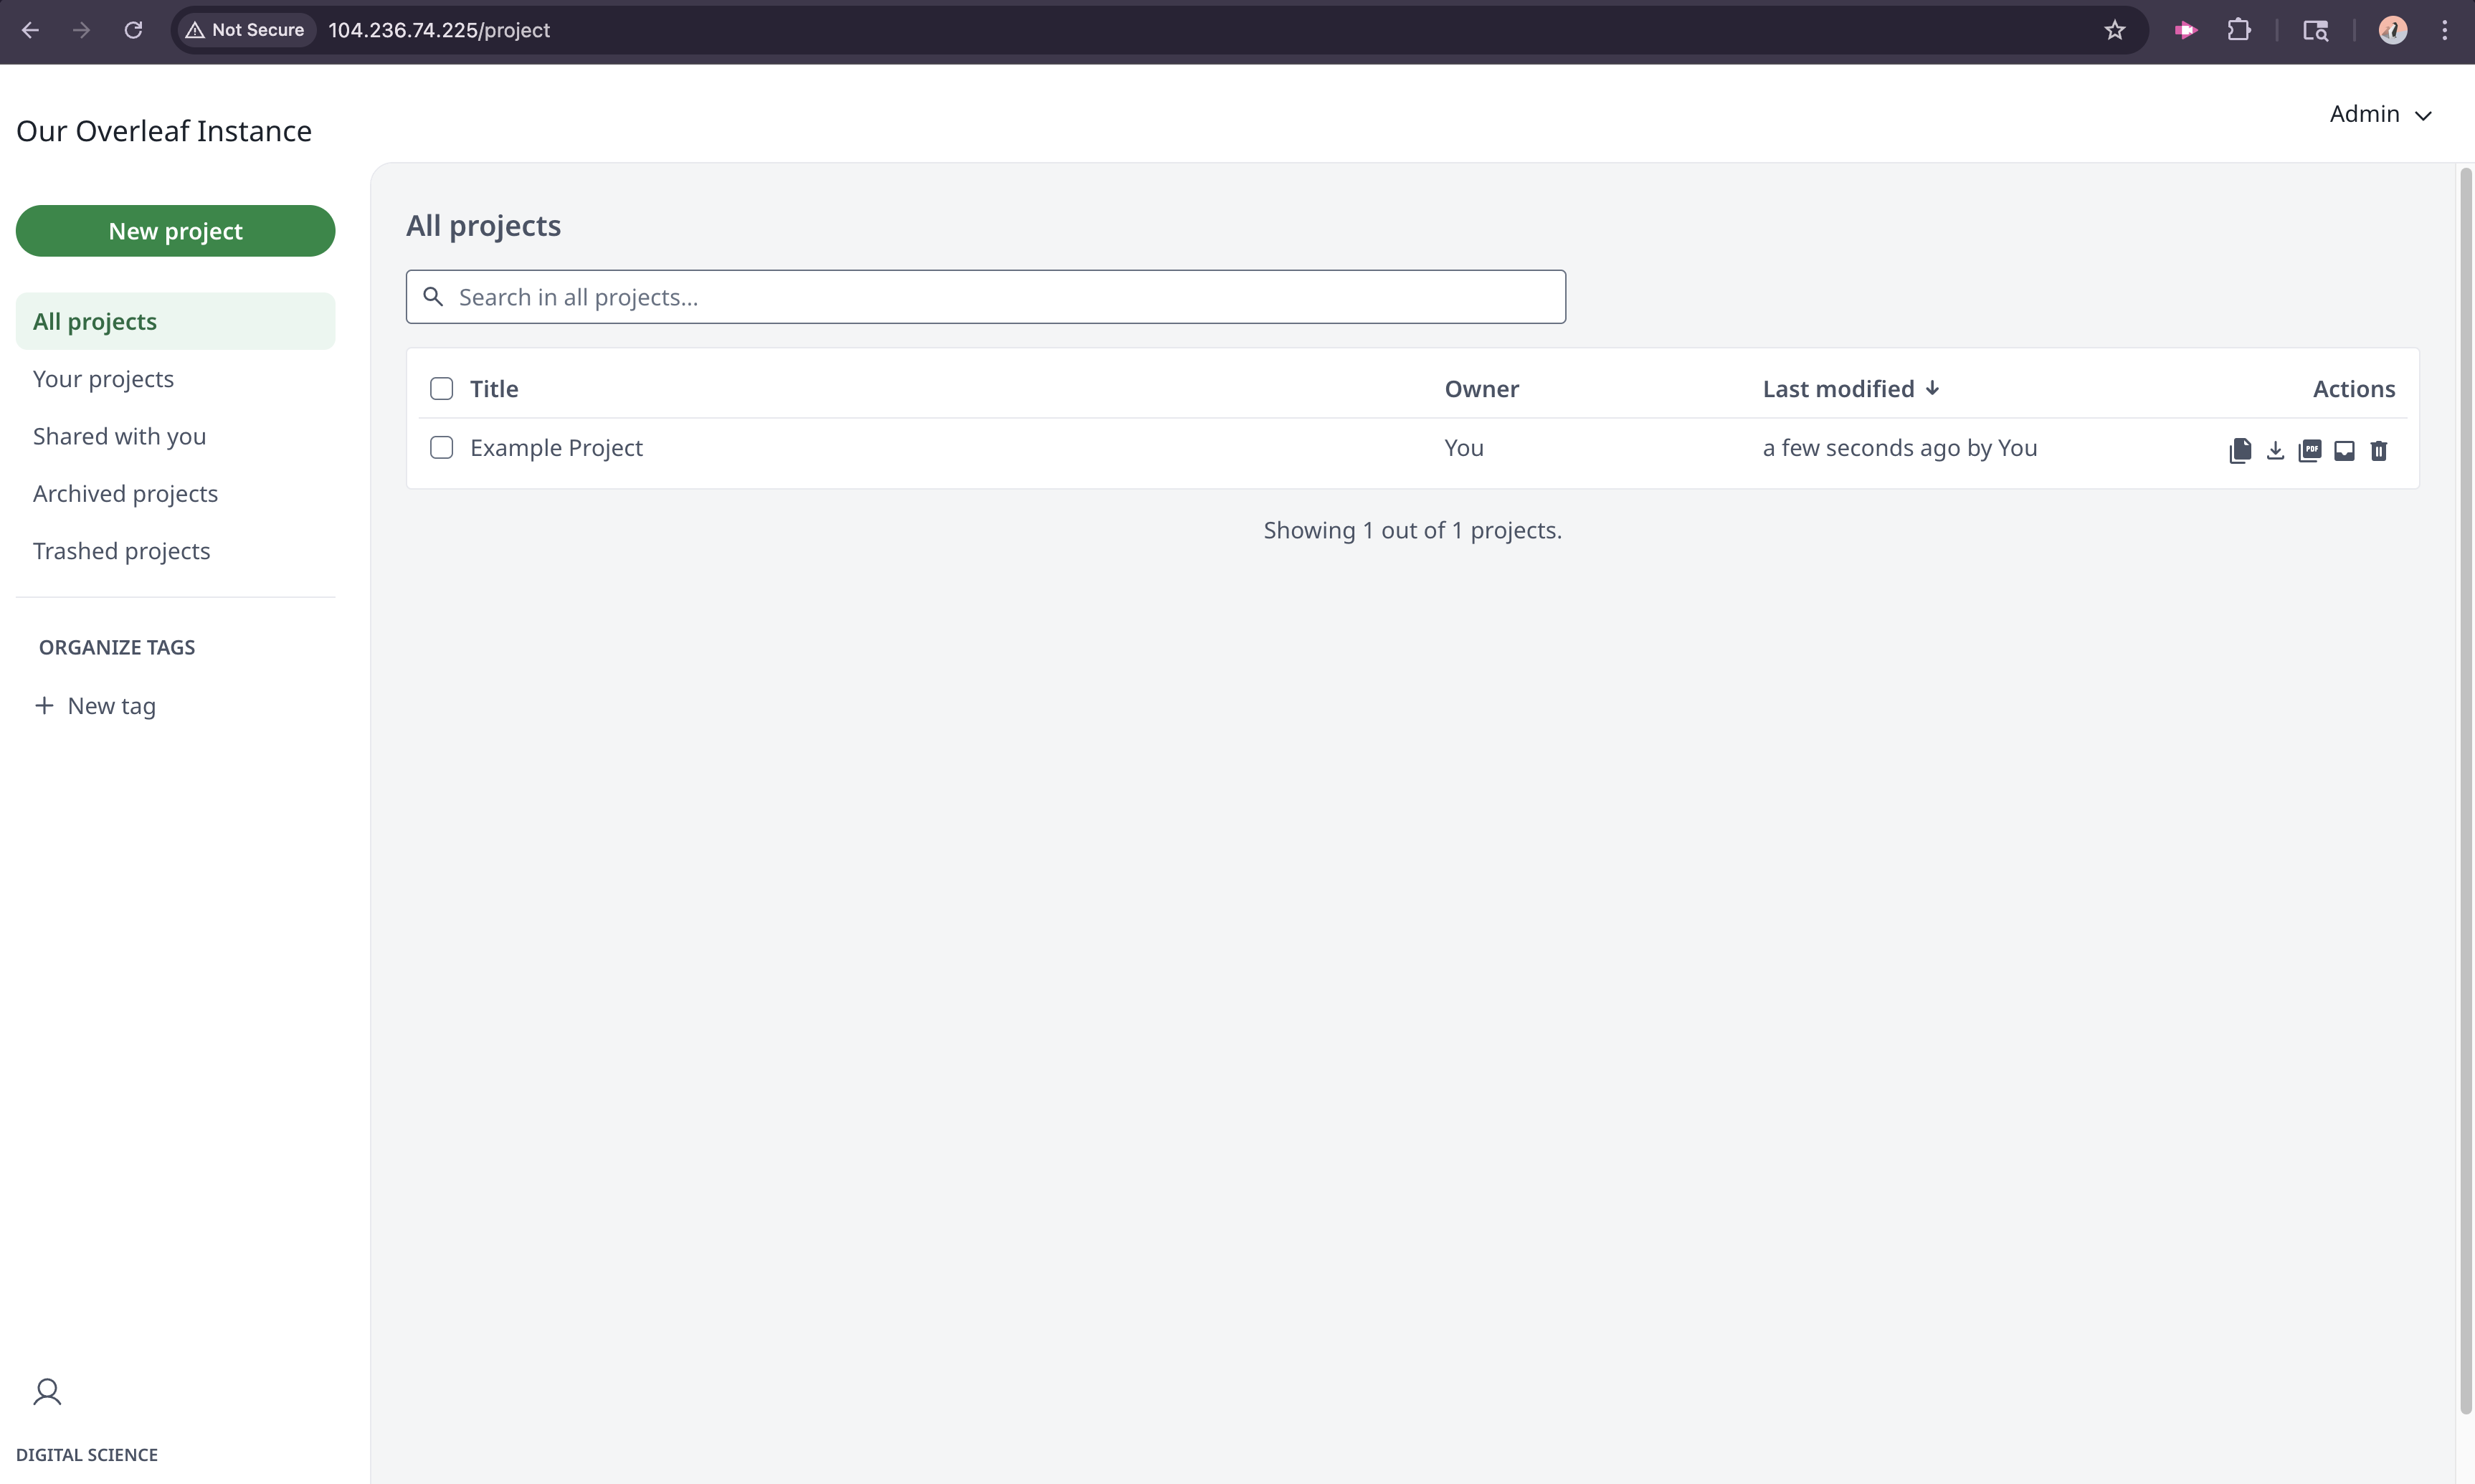
\includegraphics[width=15cm, height=10cm]{png/DigitalOcean/OverleafInstanceMainMenu.png}
    \caption{Overleaf Instance Main Menu Screenshot}
    \label{fig:OverleafInstanceMainMenu}
\end{figure}

\begin{figure}[htp]
    \centering
    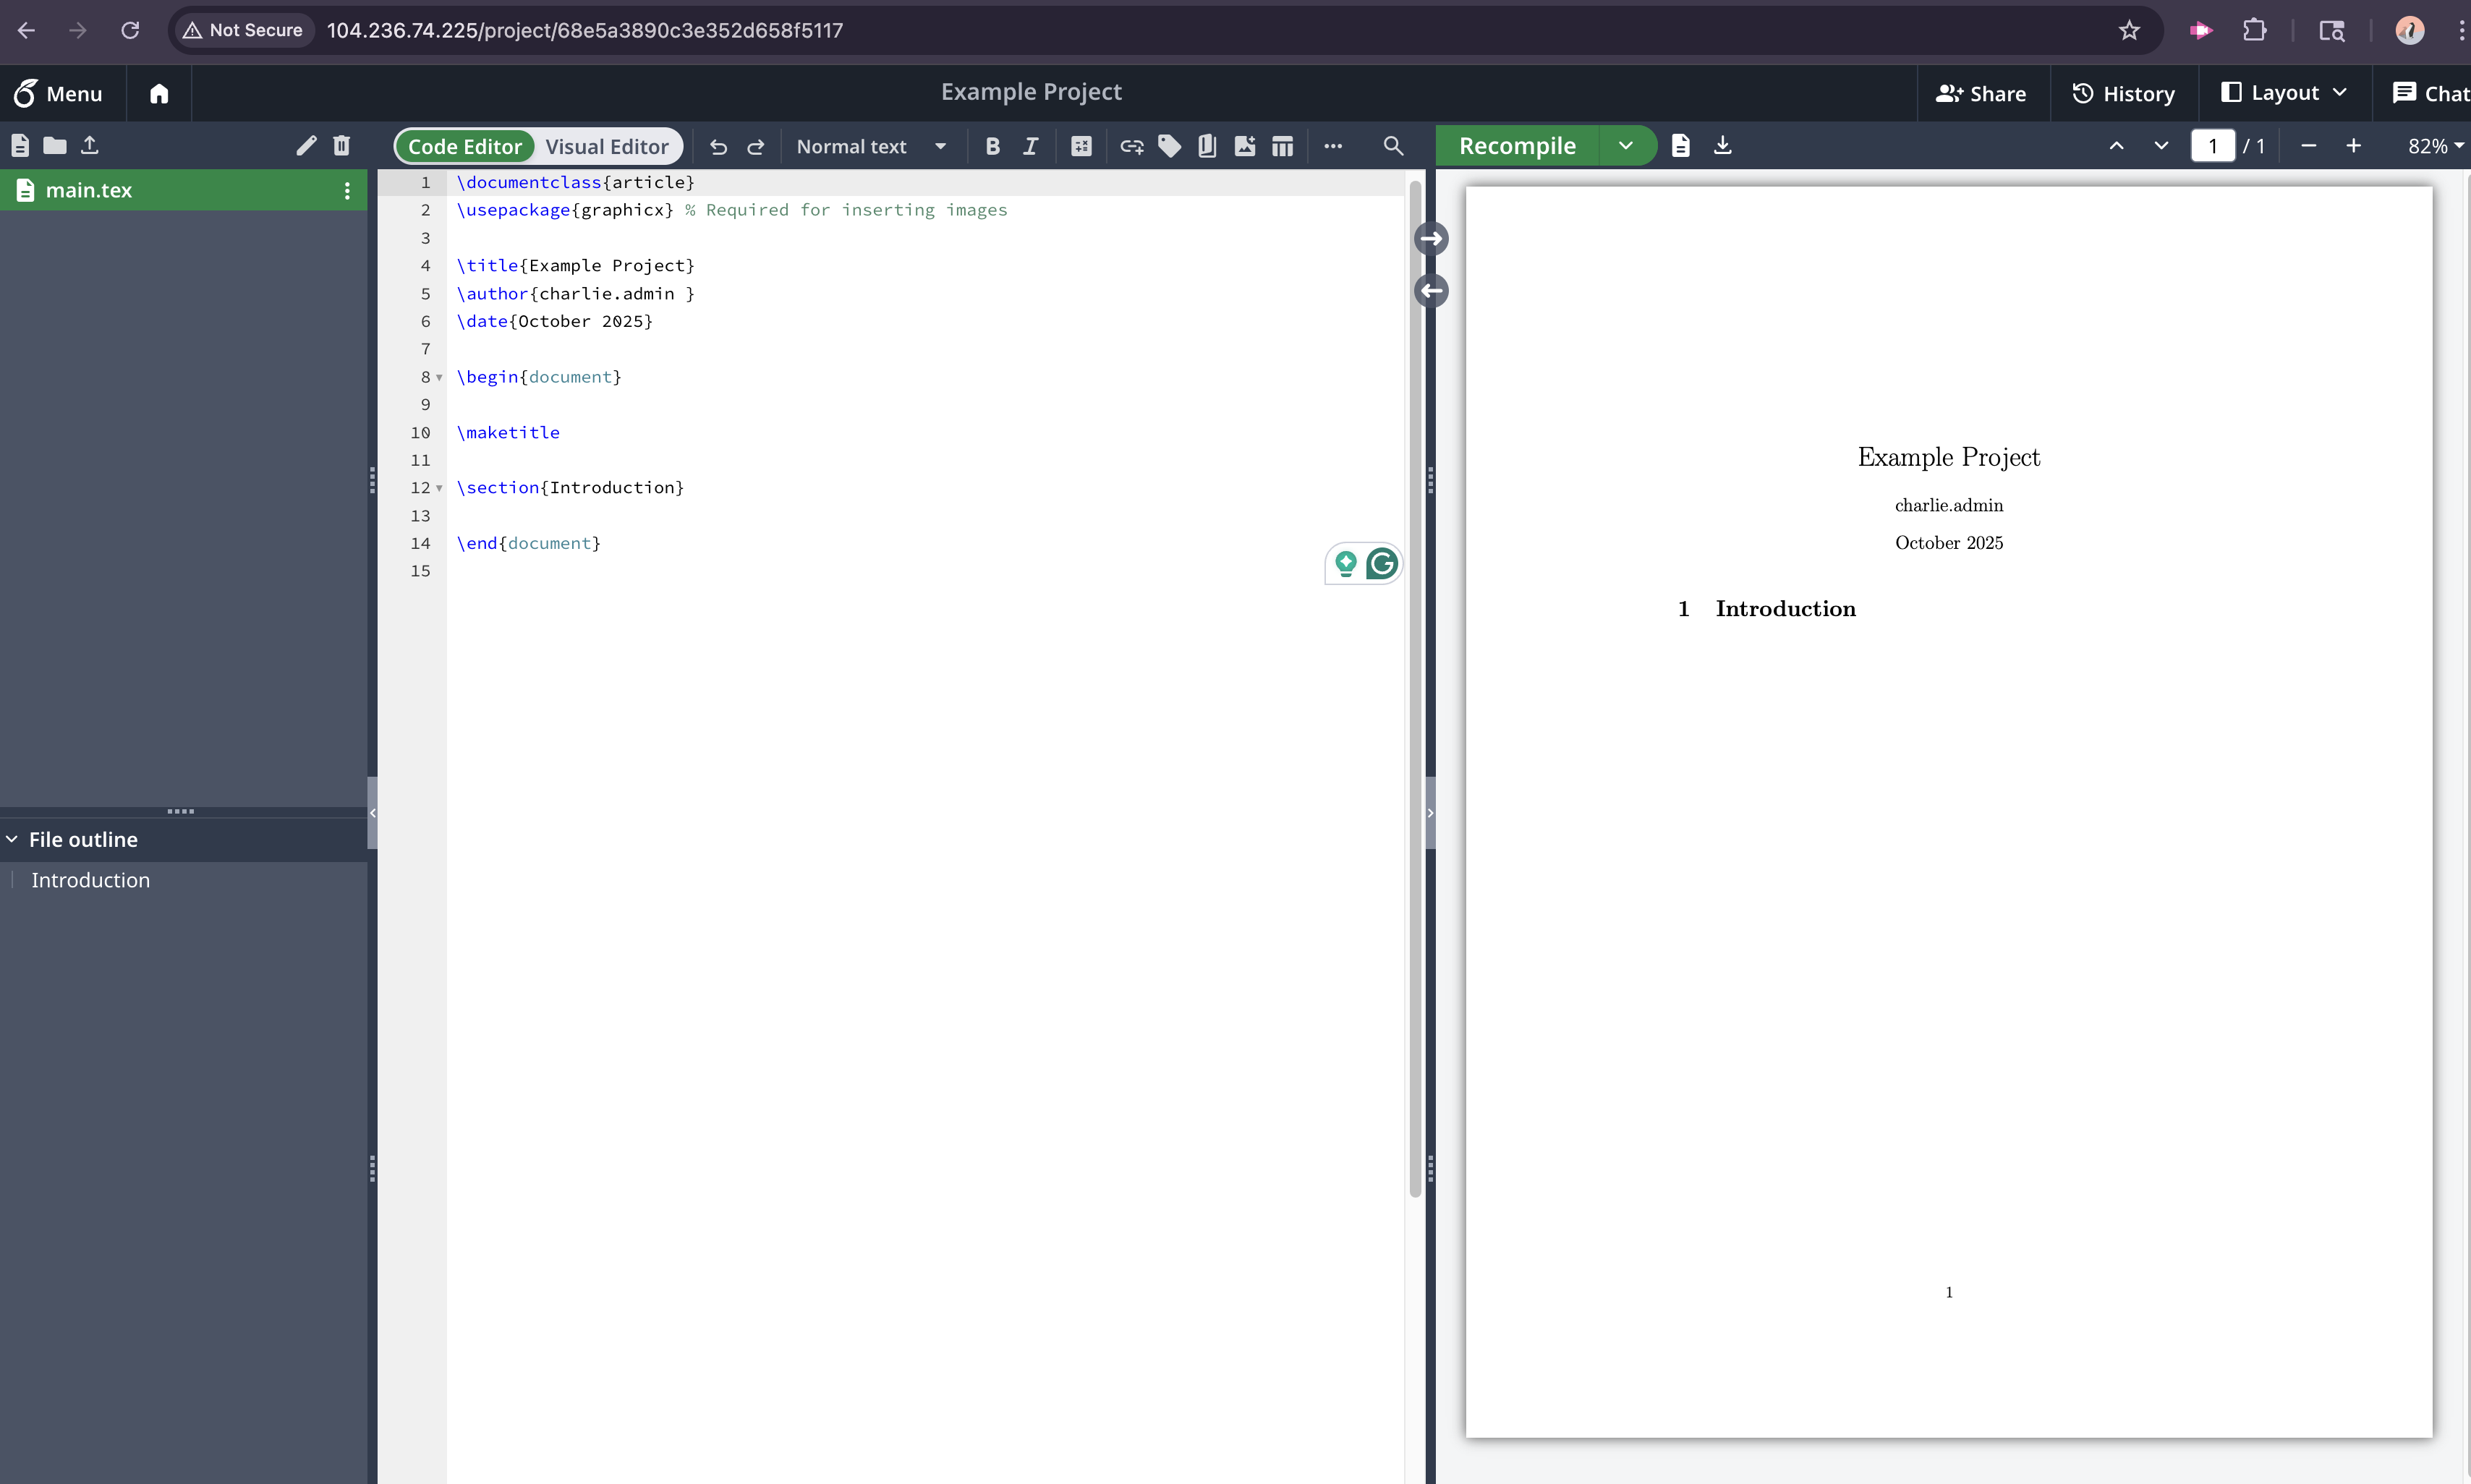
\includegraphics[width=15cm, height=10cm]{png/DigitalOcean/OverleafInstanceExProject.png}
    \caption{Overleaf Instance Example Project Screenshot}
    \label{fig:OverleafInstanceExProject}
\end{figure}